\documentclass[conference]{IEEEtran}
\usepackage{cite}
\usepackage{amsmath,amssymb,amsfonts}
\usepackage{graphicx}
\usepackage{textcomp}
\usepackage{xcolor}
\usepackage{url}
\usepackage{booktabs}
\usepackage{balance}
\emergencystretch=3em
\setlength{\textfloatsep}{7pt plus 1pt minus 1pt}
\setlength{\floatsep}{6pt plus 1pt minus 1pt}
\setlength{\intextsep}{6pt plus 1pt minus 1pt}
\def\BibTeX{{\rm B\kern-.05em{\sc i\kern-.025em b}\kern-.08em
    T\kern-.1667em\lower.7ex\hbox{E}\kern-.125emX}}
\begin{document}

\title{CryptoRegimeShift-LOB: A Crypto Level-2 Benchmark for Auditing Forecast-to-Execution Degradation}

\author{\IEEEauthorblockN{Quy Tran}
\IEEEauthorblockA{Faculty of Information Technology\\
University of Science, Ho Chi Minh City\\
Vietnam National University, Ho Chi Minh City, Vietnam\\
tvquy@fit.hcmus.edu.vn}}

\maketitle

\begin{abstract}
Limit order book (LOB) forecasting is commonly evaluated with directional metrics, but short-horizon predictive signal can degrade when it is mapped to executable decisions under spread crossing, fees, latency, visible-depth limits, and regime-dependent liquidity. This paper introduces CryptoRegimeShift-LOB, an artifact-backed benchmark and evaluation protocol for measuring forecast-to-execution degradation on full-year 2024 BTC-USDT and ETH-USDT Level-2 (L2) crypto snapshots. The protocol combines chronological purged splits, time-causal feature construction, cost-aware ternary labels, interpretable microstructure regimes, visible-depth L2 replay, fee/latency/spread/depth stress tests, day-level bootstrap uncertainty, and BTC$\leftrightarrow$ETH transfer diagnostics. Robust Selective Execution Policy (RSEP) is used only as an interpretable diagnostic gate for testing whether forecast-derived edge survives explicit cost and risk terms. Across the reported full-test baselines, results show measurable forecasting signal but consistently negative net profit and loss (PnL) after execution frictions; RSEP reduces losses in selected settings but does not establish profitability. The contribution is therefore not a new trading strategy, but a reusable applied benchmark for auditing where LOB forecasting signals fail between prediction and execution.
\end{abstract}

\begin{IEEEkeywords}
limit order book, Level-2 order book, crypto markets, market microstructure, regime shift, forecast-to-execution degradation, selective execution
\end{IEEEkeywords}

\section{Introduction}
Limit order book (LOB) forecasting is a core data mining task in high-frequency markets because the book records visible supply, demand, and liquidity at fine temporal resolution. Standard evaluation trains classifiers for future mid-price movement and reports accuracy, macro-F1, Matthews correlation coefficient (MCC), or balanced accuracy. These metrics measure predictive structure, but they do not establish whether a signal remains actionable after spread crossing, explicit fees, latency, limited visible depth, and regime-dependent liquidity. A forecast can be directionally correct while still failing along the path from prediction to execution.

This benchmark is designed for researchers and practitioners who need to audit whether a short-horizon LOB model remains useful after predictions are converted into executable decisions under observable market frictions. Instead of treating accuracy as the endpoint, the protocol records where the signal is lost: at labeling, regime exposure, replay, stress perturbation, or asset transfer.

\begin{figure*}[!t]
\centering
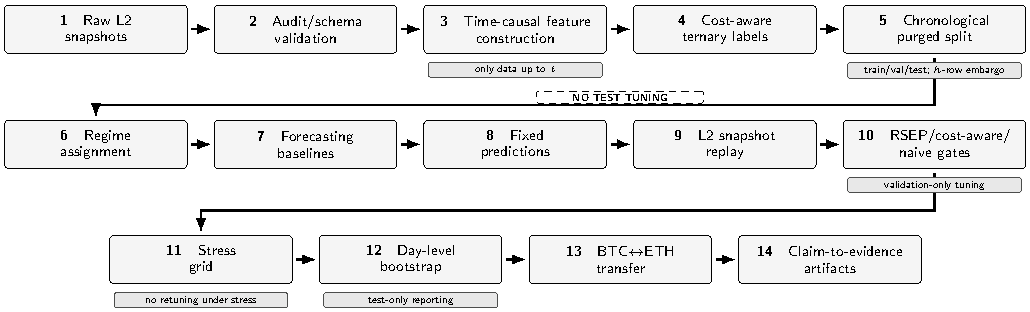
\includegraphics[width=\textwidth]{fig_1_pipeline.pdf}
\vspace{-3pt}
\caption{Overview of the CryptoRegimeShift-LOB benchmark. The protocol traces Level-2 forecasting signals from time-causal feature construction and cost-aware labeling to regime diagnostics, visible-depth replay, stress perturbations, bootstrap uncertainty, and cross-asset transfer. Training, validation, and test boundaries are preserved throughout the audit trail.}
\label{fig:pipeline}
\vspace{-6pt}
\end{figure*}


This gap is microstructural rather than purely predictive. Trading outcomes depend on trading mechanisms, liquidity provision, adverse selection, order-book depth, and the speed at which market participants react to information \cite{madhavan2000microstructure,ohara2015highfrequency,gould2013limitorderbooks}. In high-frequency settings, small timing changes or spread changes can alter the realized value of a short-horizon signal \cite{budish2015hftarmsrace,aquilina2022armsrace}. Crypto markets make this problem salient because trading is continuous, liquidity conditions can change sharply, and market-integrity concerns remain central \cite{almeida2024cryptomicrostructure,iosco_crypto2023}. A benchmark for LOB models should therefore ask not only whether a model predicts movement, but also how that signal degrades under execution frictions and changing microstructure regimes.

Recent LOB forecasting studies have substantially improved short-horizon prediction. DeepLOB and related neural approaches model spatial and temporal structure in book states \cite{deeplob2019,sirignano2019deeplob,zhang2021marketbyorder}, while benchmark and comparative studies improve experimental discipline for mid-price prediction \cite{ntakaris2018benchmark,prata2024lobbenchmark,briola2025lobframe}. However, prediction-centered evaluation leaves a downstream question underexamined: when forecasts are exposed to transaction costs, latency shifts, spread widening, depth shocks, and regime changes, how much of the apparent predictive edge survives?

CryptoRegimeShift-LOB addresses this question as an applied benchmark for tracing short-horizon LOB forecasts through observable execution frictions. The data are snapshot-level L2 observations rather than event-level L3 or market-by-order records, so the execution layer uses a visible-depth market-order replay approximation. This boundary keeps the benchmark focused on auditable degradation analysis while reserving hidden liquidity, queue position, passive fills, and live venue behavior for future data settings.

The paper makes four benchmark-first applied contributions.
\begin{itemize}
\setlength\itemsep{0pt}
\item \textbf{Full-year Level-2 crypto benchmark.} We construct BTC-USDT and ETH-USDT snapshot-level L2 datasets with chronological purged splits, time-causal feature construction, and auditable split manifests.
\item \textbf{Cost-aware labels and regimes.} We define ternary labels using local spread and fee proxies, and assign interpretable microstructure regimes for by-regime forecasting and execution diagnostics.
\item \textbf{Forecast-to-execution evaluation.} We map fixed predictions into visible-depth L2 replay, validation-selected execution gates, fee/latency/spread/depth stress tests, and day-level bootstrap uncertainty.
\item \textbf{Failure-oriented probes.} We use RSEP and BTC$\leftrightarrow$ETH transfer to expose where forecast-derived signal degrades under costs, regimes, and asset shift.
\end{itemize}
RSEP is therefore not the main algorithmic novelty. It is one probe inside a reusable evaluation path whose purpose is to expose failure modes that prediction-only LOB benchmarks hide.

Figure~\ref{fig:pipeline} summarizes the resulting audit trail. Each stage preserves chronological boundaries, so reported degradation can be traced from data construction to forecasting, replay, stress testing, and transfer diagnostics. The benchmark separates predictive structure, local cost clearance, and execution stress; positive gross directional movement with negative net PnL becomes localized evidence about where an apparent signal fails rather than merely a lower leaderboard score.

\section{Related Work}
\subsection{LOB Forecasting and Benchmarks}
LOB forecasting has been studied as short-horizon mid-price movement prediction. FI-2010 standardized supervised LOB prediction \cite{ntakaris2018benchmark}; DeepLOB showed that convolutional and recurrent layers can extract book structure \cite{deeplob2019}; and later work expanded deep, market-by-order, and transformer-style models \cite{sirignano2019deeplob,zhang2021marketbyorder,xiao2025lit}. Recent benchmark and microstructural guide papers emphasize rigorous comparison and feature interpretation \cite{prata2024lobbenchmark,briola2025lobframe}. These works motivate our forecasting baselines, but our novelty is the execution-aware evaluation path, not a new predictor.

LOB models are sensitive to horizon, label threshold, class balance, and visible depth. CryptoRegimeShift-LOB therefore treats forecasting models as signal generators and evaluates whether their signals survive labels, regimes, and replay, rather than presenting a predictor leaderboard.

\subsection{Market Microstructure and Execution Frictions}
Market microstructure research shows that observed prices and realized trading outcomes depend on trading rules, visible and hidden liquidity, order flow, and adverse selection \cite{madhavan2000microstructure,ohara2015highfrequency,cont2010stochasticlob,cartea2015algorithmic}. HFT research further shows that latency and speed are economically meaningful frictions rather than implementation details \cite{budish2015hftarmsrace,aquilina2022armsrace,aquilina2025speedpremium}. For LOB forecasting, this implies that directional correctness is not enough: a signal must survive spread crossing, fee, depth, and timing risk. Because our data are L2 snapshots, we evaluate only a visible-depth market-order approximation and explicitly avoid L3 or live-execution claims.

Crypto L2 data intensifies this distinction. Snapshot data records visible price levels and sizes, which is sufficient to construct spread, depth, imbalance, and market-order sweep approximations. It does not record the complete order lifecycle. Therefore, the benchmark is deliberately conservative: it evaluates costs observable from visible depth and stress perturbations, while treating unobserved queue priority, cancellation races, and hidden liquidity as outside scope. This makes the empirical claims narrower but more defensible.

\subsection{Regime-Aware and Stress Evaluation}
Aggregate test metrics can hide failures under distribution shift. Robustness and dataset-shift studies show that fixed test performance can degrade under shifted conditions \cite{quinonero2009datasetshift,ovadia2019uncertainty,koh2021wilds}. Time-series evaluation also requires chronological validation to avoid leakage and overoptimistic estimates \cite{bergmeir2018timeseriescv,cerqueira2020timeserieseval}. Financial evaluation adds cost and data-snooping risks, motivating bootstrap and conservative backtest interpretation \cite{efron1979bootstrap,politis1994stationarybootstrap,white2000realitycheck,bailey2016backtestoverfitting,lopezdeprado2018afml}. CryptoRegimeShift-LOB combines these ideas in a domain-specific path: time-causal L2 features $\rightarrow$ cost-aware labels $\rightarrow$ regime-aware forecasting $\rightarrow$ execution replay $\rightarrow$ stress testing and cross-asset diagnostics.

\section{Data and Benchmark Construction}
\subsection{L2 Snapshot Data}
The benchmark uses Binance BTC-USDT and ETH-USDT L2 order book snapshots for 2024, following the Crypto Lake data documentation for historical crypto market data \cite{cryptolake_data}. Each row is a snapshot with 20 bid levels and 20 ask levels, represented by price and size fields, along with timestamp, sequence, exchange, and symbol metadata. The audit-level dataset contains 167,753,156 valid BTC-USDT snapshots and 114,416,283 valid ETH-USDT snapshots over 366 calendar days. After dropping rows that lack the required future horizon for labels, the feature/label stores contain 167,751,306 BTC-USDT rows and 114,414,433 ETH-USDT rows.

\begin{table*}[t]
\centering
\caption{Chronological split audit for fixed purged benchmark artifacts. Validation is explicit; test is reserved for final reporting. Row counts exclude the $h=50$ embargo rows before validation and test boundaries.}
\label{tab:data_split}
\scriptsize
\begin{tabular}{@{}p{0.10\linewidth}p{0.18\linewidth}p{0.18\linewidth}p{0.18\linewidth}p{0.20\linewidth}@{}}
\toprule
Symbol & Train & Validation & Test & Boundary audit \\
\midrule
BTC-USDT & 100,650,733 rows; Jan 1--Aug 31 & 33,550,211 rows; Aug 31--Oct 28 & 33,550,262 rows; Oct 28--Dec 31 & $h=50$ embargo; no label-window overlap \\
ETH-USDT & 68,648,609 rows; Jan 1--Sep 9 & 22,882,837 rows; Sep 9--Nov 4 & 22,882,887 rows; Nov 4--Dec 31 & $h=50$ embargo; no label-window overlap \\
\bottomrule
\end{tabular}
\end{table*}

\subsection{Audit, Causal Features, and Labels}
Before feature construction, snapshots are audited for schema validity, timestamp validity, positive price and size fields, and non-crossed best quotes. These checks create a data version that can be linked to later forecasting, execution, stress, and bootstrap artifacts. The audit does not reconstruct unobserved message-level events; rows with invalid book states are cleaned or logged under the benchmark configuration.

For each decision time $t$, features use only information available at or before $t$. Let $b^{p}_{t,\ell},b^{q}_{t,\ell}$ be bid price and size at level $\ell$, and let $a^{p}_{t,\ell},a^{q}_{t,\ell}$ be ask price and size. The mid-price and spread are
\begin{equation}
m_t=\frac{a^{p}_{t,0}+b^{p}_{t,0}}{2},\qquad s_t=a^{p}_{t,0}-b^{p}_{t,0}.
\end{equation}
The feature store contains spread, relative spread, multi-level depth, imbalance, order-flow-imbalance proxies, short-horizon returns and volatility, momentum, choppiness, liquidity-stress scores, and adverse-selection proxies. Rolling statistics end at $t$; feature scalers and model parameters are fitted on training rows, regime quantiles are fitted on the training prefix, policy thresholds are tuned on validation rows, and test rows are not used for fitting or selection.

Labels are cost-aware ternary targets. For horizon $h$,
\begin{equation}
r_{t,h}=\frac{m_{t+h}-m_t}{m_t+\epsilon},\qquad
 y_t=\begin{cases}
\mathrm{UP}, & r_{t,h}>\tau_t,\\
\mathrm{DOWN}, & r_{t,h}< -\tau_t,\\
\mathrm{FLAT}, & \mathrm{otherwise},
\end{cases}
\end{equation}
where $\epsilon=10^{-9}$. The benchmark uses a fixed local threshold
\begin{equation}
\tau_t=(1+\kappa)\rho_t+\frac{f}{10000},\qquad
\rho_t=\frac{s_t}{m_t+\epsilon}.
\label{eq:label_threshold}
\end{equation}
The default benchmark constants are $h=50$ events, $f=1.0$ bps, and $\kappa=0.5$, so $\tau_t=1.5\rho_t+0.0001$. The same constants are used for BTC-USDT and ETH-USDT. They are fixed in the benchmark configuration before any split is evaluated; they are not fitted, validation-tuned, or adjusted using test data. The inequalities are strict: equality with either boundary is assigned to FLAT.

\begin{table}[t]
\centering
\caption{Default benchmark configuration for cost-aware labels. Label thresholds are fixed from configuration and are not selected on the test split.}
\label{tab:benchmark_config}
\scriptsize
\begin{tabular}{@{}p{0.27\linewidth}p{0.29\linewidth}p{0.34\linewidth}@{}}
\toprule
Quantity & Default & Role \\
\midrule
Horizon $h$ & 50 events & Future mid-price return horizon \\
Return $r_{t,h}$ & $(m_{t+h}-m_t)/(m_t+\epsilon)$ & Supervised target return \\
Relative spread $\rho_t$ & $s_t/(m_t+\epsilon)$ & Snapshot-local cost proxy \\
Fee $f$ & 1.0 bps & Explicit label friction proxy \\
Slippage multiplier $\kappa$ & 0.5 & Spread-proportional buffer \\
Threshold $\tau_t$ & $(1+\kappa)\rho_t+f/10000$ & UP/DOWN significance boundary \\
Trade size $q$ & Not used & Simulator-only parameter \\
Latency/depth sweep & Not used & Simulator-only parameters \\
Asset constants & None & Shared across BTC-USDT and ETH-USDT \\
\bottomrule
\end{tabular}
\end{table}

This design makes the FLAT class meaningful: it is not a residual class for uncertain predictions, but a statement that the future move is too small to clear the fixed local cost proxy. Therefore, UP and DOWN labels represent movements that are directionally and cost-aware significant under the chosen horizon. Trade size, latency, and visible-depth sweep are deliberately excluded from $\tau_t$; they enter only later in the execution simulator. The label threshold is a one-step local significance proxy; full round-trip fees and visible-depth effects are applied only in execution replay.

The future return is used only to define the supervised target, not as a feature, regime input, normalization input, or policy decision variable. All reported benchmark artifacts use chronological purged splits: training fits model parameters, feature scalers, and regime quantiles; validation tunes model-selection thresholds, execution thresholds, and RSEP parameters; and test is reserved for final reporting. Because the label uses a future horizon of $h=50$ events, the split generator excludes the last $h$ rows before the train--validation boundary and the last $h$ rows before the validation--test boundary. These embargoed rows are excluded from model fitting, validation tuning, execution replay, stress-grid evaluation, and bootstrap reporting. Thus, no row whose label window crosses a later split boundary is used in the reported train, validation, or test artifacts. All forecasting, execution, stress-grid, bootstrap, and cross-asset tables in this submission were regenerated after applying the $h$-row embargo; artifact hashes and split manifests are included in the supplementary artifact release.

\section{Regimes and Forecasting Baselines}
\subsection{Microstructure Regime Taxonomy}
The regime taxonomy is a diagnostic lens, not an oracle market-state model. A deterministic assignment function maps time-causal diagnostics to regimes,
\begin{equation}
\begin{split}
r^{\rm reg}_t &= g(\mathbf{z}_t),\quad r^{\rm reg}_t\in\mathcal{R},\\
\mathbf{z}_t &= [z^{\rm spread}_t,z^{\rm depth}_t,z^{\rm imb}_t,z^{\rm vol}_t,\\
 z^{\rm mom}_t,z^{\rm chop}_t,z^{\rm liq}_t,z^{\rm adv}_t].
\end{split}
\end{equation}

The full artifact taxonomy contains 11 priority labels. In the main paper we report five compressed diagnostic groups to save space while keeping the time-causal construction auditable.

\begin{table}[t]
\centering
\caption{Compressed diagnostic regime groups. Full priority rules, thresholds, counts, and sensitivity checks are released as artifacts.}
\label{tab:regime_taxonomy}
\scriptsize
\begin{tabular}{p{0.35\linewidth}p{0.55\linewidth}}
\toprule
Group & Diagnostic role \\
\midrule
Liquidity stress & Drought or moderate depth/spread deterioration. \\
Volatile states & High volatility under liquid or illiquid visible depth. \\
Momentum/adverse states & Directional pressure and adverse-selection risk. \\
Choppy/recovery states & Reversal-prone or post-shock transition snapshots. \\
Calm/transition/unknown & Low-stress, residual, or ambiguous observations. \\
\bottomrule
\end{tabular}
\end{table}

The taxonomy audit reports \texttt{UNKNOWN} explicitly: BTC-USDT has 13.19\% overall \texttt{UNKNOWN} share and ETH-USDT has 12.68\%; alternative quantile settings change UNKNOWN rates but keep roughly 86\% agreement with the baseline taxonomy. These sensitivity results are diagnostic and are not used to retune thresholds on test data.

By-regime evaluation is necessary because a model can look acceptable under an aggregate macro-F1 or MCC while concentrating errors, cost, or turnover in unfavorable states. Execution metrics are even more regime-sensitive because spread, available depth, and latency penalties are not constant across market conditions. A signal that is marginal in a calm liquid book may be dominated by adverse selection or cost in a momentum-toxic or liquidity-drought state. Thus, the taxonomy provides a bridge from prediction metrics to selective-execution diagnostics: if a policy reduces exposure in some regimes but fails in others, the mixed result is treated as evidence rather than hidden.

\subsection{Forecasting Baselines}
The benchmark is not intended to declare architecture leadership. Forecasting models are controlled signal generators for downstream degradation analysis; the tabular XGBoost baseline and temporal convolutional baseline are included for controlled comparison rather than leaderboard claims \cite{chen2016xgboost,bai2018tcn}. Main claims are restricted to models with fixed full-test prediction and replay artifacts. Table~\ref{tab:baseline_coverage} makes the coverage explicit. DeepLOB-style CNN--LSTM is included through a fixed purged controlled subsample because it is a canonical LOB architecture \cite{deeplob2019,briola2025lobframe}; the lightweight Transformer remains an implementation sanity check \cite{xiao2025lit}.

\begin{table}[t]
\centering
\caption{Baseline coverage. Main execution claims use only fixed full-test prediction and replay artifacts; partial neural baselines are reported as coverage checks.}
\label{tab:baseline_coverage}
\scriptsize
\setlength{\tabcolsep}{2pt}
\begin{tabular}{p{0.30\linewidth}p{0.20\linewidth}p{0.38\linewidth}}
\toprule
Model family & Replay? & Role in paper \\
\midrule
SGD & yes & Diagnostic linear control with fixed full-test replay \\
XGBoost & yes & Strong tabular nonlinear baseline with fixed full-test replay \\
TCN & yes & Temporal neural baseline and stride-1 negative evidence \\
DeepLOB CNN--LSTM & no & Canonical LOB architecture on a purged controlled subsample \\
Lightweight Transformer & no & Sequence implementation sanity check only \\
\bottomrule
\end{tabular}
\end{table}

The DeepLOB controlled subsample uses the purged BTC source with 100k train, 25k validation, and 50k test windows; it reports accuracy 0.4367, macro-F1 0.3483, MCC 0.0221, and balanced accuracy 0.3487. Because this result is forecasting-only and not fixed full-test replay-ready, it is not used to compare execution policies. It is included only to document architectural interface coverage and to prevent the benchmark from being presented as a tabular-only evaluation.

Forecasting performance is reported with accuracy, macro-F1, MCC, and balanced accuracy because the ternary task is class-imbalanced. Table~\ref{tab:forecasting} shows that rankings depend on the metric: XGBoost has the highest accuracy, stride-1 TCN has the strongest macro-F1 among full-test comparable baselines, and the tabular models remain competitive under MCC.

\begin{table}[t]
\centering
\caption{Held-out forecasting metrics. Prediction quality is necessary but not sufficient for execution value.}
\label{tab:forecasting}
\footnotesize
\begin{tabular}{lrrrr}
\toprule
Model & Acc. & Macro-F1 & MCC & Bal. Acc. \\
\midrule
SGD & 0.5589 & 0.4652 & 0.2363 & 0.4637 \\
XGBoost & 0.5677 & 0.4562 & 0.2364 & 0.4555 \\
TCN stride-10 & 0.5282 & 0.4689 & 0.2275 & 0.4692 \\
TCN stride-1 & 0.5281 & 0.4688 & 0.2274 & 0.4691 \\
\bottomrule
\end{tabular}
\end{table}

The stride-1 TCN is important negative evidence: macro-F1 alone would make it look strongest, but its downstream selective-execution result does not support a universal RSEP advantage over the cost-aware threshold. Thus, forecasting metrics are diagnostics, not deployment evidence; the next section tests whether the same predictions survive cost-aware replay.

\section{Forecast-to-Execution Evaluation}
\subsection{L2 Snapshot Replay Specification}
The execution layer converts predicted actions into market-order-style replay against visible L2 depth. This replay is a benchmark approximation: it does not model passive queue priority, hidden liquidity, cancellation races, venue routing, or live latency. Spread crossing is implicit because buys execute on ask levels and sells execute on bid levels.

For a nonzero signal at row $i$, entry occurs at $i+\ell$ where $\ell$ is the configured latency in event rows, and exit occurs after the label horizon. The requested quantity at a replay snapshot is
\begin{equation}
q_t^*=\frac{N}{\max(m_t,\epsilon)},
\end{equation}
where $N$ is the configured trade notional, $m_t$ is the snapshot mid-price, and $\epsilon=10^{-9}$. A market buy sweeps asks from level $0$ to level $19$; a market sell sweeps bids in the same level order. Under spread and depth stress, the executable prices and visible sizes are
\begin{align}
p^{\rm buy}_{t,l}&=m_t+\alpha(p^{\rm ask}_{t,l}-m_t), &
d^{\rm buy}_{t,l}&=\beta d^{\rm ask}_{t,l},\\
p^{\rm sell}_{t,l}&=m_t-\alpha(m_t-p^{\rm bid}_{t,l}), &
d^{\rm sell}_{t,l}&=\beta d^{\rm bid}_{t,l},
\end{align}
where $\alpha$ is the spread multiplier and $\beta$ is the depth multiplier. At each level, the fill is $x_l=\min(q_{\rm remaining},\max(d_{t,l},0))$. Nonfinite, nonpositive, or absent deeper-level price/size values are treated as unavailable depth for that level.

The execution price is the visible-depth VWAP,
\begin{equation}
\mathrm{VWAP}_t=\frac{\sum_l x_l p_{t,l}}{\sum_l x_l},
\end{equation}
with fill ratio $\sum_l x_l/q_t^*$. If \texttt{partial\_fill=true}, a trade is kept only when both entry and exit fill ratios are at least the configured \texttt{min\_fill\_ratio}; if \texttt{partial\_fill=false}, any non-full sweep is converted to a zero fill and skipped. The matched trade quantity is the smaller of entry and exit filled quantities.

Fees are charged on matched filled notional, not requested notional:
\begin{equation}
C=\frac{f}{10000}\left(q p_{\rm entry}+q p_{\rm exit}\right),
\end{equation}
where $f$ is the fee in basis points. Long gross PnL is $q(p_{\rm exit}^{\rm sell}-p_{\rm entry}^{\rm buy})$; short gross PnL is $q(p_{\rm entry}^{\rm sell}-p_{\rm exit}^{\rm buy})$; net PnL subtracts $C$. Required replay columns are validated before simulation. Rows with nonfinite or nonpositive mid-price, invalid best prices or sizes, or crossed best books are treated as zero-fill rows. These rules specify depth exhaustion, fee application, latency indexing, and partial fills directly from L2 snapshots.

The execution layer evaluates three decision mappings. The naive threshold policy trades when the predicted UP or DOWN probability exceeds a validation-tuned threshold. The cost-aware threshold policy estimates whether expected directional return exceeds spread, fee, and depth-slippage proxies. RSEP adds an inspectable diagnostic comparison against explicit latency, liquidity, adverse-selection, and regime-risk terms. The RSEP $\lambda$ coefficients are fixed benchmark constants, while $\theta$ is selected on validation data. The held-out test split is used only for final reporting and is not used to choose favorable execution assumptions.

\subsection{RSEP Gate}
RSEP gates a forecast-derived action by comparing forecast-implied expected edge with explicit cost and risk terms. Let $\mu_y$ denote the training-split mean future return for class $y\in\{\textsc{Up},\textsc{Flat},\textsc{Down}\}$, and let $p_t(y)$ be the forecast probability at time $t$. The implementation uses
\begin{equation}
\widehat{e}_t=
p_t(\textsc{Up})\mu_{\textsc{Up}}+
p_t(\textsc{Flat})\mu_{\textsc{Flat}}+
p_t(\textsc{Down})\mu_{\textsc{Down}}.
\label{eq:rsep_edge}
\end{equation}
This diagnostic edge uses train-split class-return means; it is not a calibrated live expected-return model. RSEP is intentionally named to make the diagnostic policy reproducible; it should not be read as a proposed trading algorithm. Calibration and cross-asset distribution shifts are treated as degradation diagnostics, and ECE summaries are included in the supplementary artifact release.
The cost term is $\widehat{c}_t=\rho_t+f/10000$, where $\rho_t$ is relative spread and $f$ is the simulator fee in basis points. The gate trades only if
\begin{equation}
\widehat{e}_t>
\widehat{c}_t+
\lambda_{\rm lat}\widehat{r}^{\rm lat}_t+
\lambda_{\rm liq}\widehat{r}^{\rm liq}_t+
\lambda_{\rm adv}\widehat{r}^{\rm adv}_t+
\lambda_{\rm reg}\widehat{r}^{\rm reg}_t+\theta.
\label{eq:rsep}
\end{equation}
This gate is intentionally simple: its role is to make cost and risk assumptions inspectable, not to maximize trading performance.
For negative edge, the symmetric short rule is used: sell if $\widehat{e}_t<-\widehat{E}^{\rm req}_t$, where $\widehat{E}^{\rm req}_t$ is the right-hand side of Eq.~\eqref{eq:rsep}. Otherwise the policy abstains. Equality abstains because both comparisons are strict. RSEP is not a forecasting model or universal trading policy; it is a diagnostic gate for testing whether explicit cost/risk terms reduce adverse exposure.

\begin{table}[t]
\centering
\caption{RSEP gate specification. The table exposes the fixed decision rule used in replay; it is a diagnostic gate rather than a learned trading algorithm.}
\label{alg:rsep_gate}
\scriptsize
\begin{tabular}{p{0.28\linewidth}p{0.62\linewidth}}
\toprule
Component & Specification \\
\midrule
Inputs & Forecast probabilities $p_t$, train class-return means $\mu$, spread $\rho_t$, fee $f$, risk scores, regime label, fixed $\lambda$, and validation-selected $\theta$. \\
Edge & Compute $\widehat{e}_t=\sum_y p_t(y)\mu_y$. \\
Cost & Set $\widehat{c}_t=\rho_t+f/10000$. \\
Risk & Use latency, liquidity-drought, adverse-selection, and regime penalties; regime risk is mapped from liquidity drought $1.0$ to choppy mean-reverting $0.25$, and $0$ otherwise. \\
Required edge & $\widehat{E}^{\rm req}_t=\widehat{c}_t+\lambda_{\rm lat}r^{\rm lat}_t+\lambda_{\rm liq}r^{\rm liq}_t+\lambda_{\rm adv}r^{\rm adv}_t+\lambda_{\rm reg}r^{\rm reg}_t+\theta$. \\
Decision & Buy if $\widehat{e}_t>\widehat{E}^{\rm req}_t$, sell if $\widehat{e}_t<-\widehat{E}^{\rm req}_t$, and abstain otherwise; equality also abstains. \\
\bottomrule
\end{tabular}
\end{table}

\subsection{Execution Results}
Table~\ref{tab:execution} reports the main forecast-to-execution comparison. All reported policies remain net negative after costs. For SGD and XGBoost, RSEP mitigates losses relative to the cost-aware threshold in selected settings, but the improvement is relative loss mitigation. The stride-1 TCN case is important because it shows RSEP is not uniformly better than the cost-aware threshold. This directly blocks any claim that a stronger macro-F1 automatically yields better selective execution.

\begin{table*}[t]
\centering
\caption{Forecast-to-execution comparison with day-level bootstrap confidence intervals on the held-out test split. Net PnL remains negative under the replay assumptions; results localize degradation rather than establish deployable trading performance.}
\label{tab:execution}
\scriptsize
\begin{tabular}{llrrcc}
\toprule
Model & Policy & Trades & Days & Net PnL [95\% CI] & Net/trade [95\% CI] \\
\midrule
SGD & Naive & 32,891 & 65 & -4,557.58 [-5,228.91, -3,835.79] & -0.1386 [-0.1465, -0.1313] \\
SGD & Cost-aware & 67,165 & 65 & -8,891.63 [-9,950.32, -7,735.22] & -0.1324 [-0.1373, -0.1279] \\
SGD & RSEP-full & 33,713 & 65 & -4,437.49 [-5,016.42, -3,821.41] & -0.1316 [-0.1361, -0.1270] \\
XGBoost & Naive & 880,927 & 65 & -115,238.26 [-133,871.64, -98,314.48] & -0.1308 [-0.1331, -0.1284] \\
XGBoost & Cost-aware & 37,945 & 65 & -4,494.39 [-5,103.67, -3,926.69] & -0.1184 [-0.1216, -0.1151] \\
XGBoost & RSEP-full & 36,360 & 65 & -4,303.19 [-4,843.66, -3,796.91] & -0.1183 [-0.1215, -0.1152] \\
TCN stride-1 & Naive & 19,932 & 65 & -3,355.28 [-4,897.41, -2,009.46] & -0.1683 [-0.1880, -0.1484] \\
TCN stride-1 & Cost-aware & 4,570 & 65 & -788.00 [-1,124.94, -500.53] & -0.1724 [-0.2159, -0.1429] \\
TCN stride-1 & RSEP-full & 5,435 & 65 & -814.17 [-1,041.07, -609.71] & -0.1498 [-0.1605, -0.1367] \\
\bottomrule
\end{tabular}
\end{table*}

Two observations matter. First, positive gross PnL does not survive costs, which is why prediction-only evaluation is incomplete. Second, lower turnover can reduce total losses, but must be read with net PnL, per-trade loss, regime exposure, and day-level uncertainty. RSEP is evaluated as a diagnostic gate, not a profit-maximizing optimizer. The paired day-level bootstrap artifact shows that RSEP minus cost-aware is positive for SGD and XGBoost, but crosses zero for TCN stride-1. These differences support only relative loss mitigation because absolute net PnL remains negative.

Ablation artifacts are interpreted with restraint. Removing latency, liquidity, adverse-selection, or regime components generally worsens net PnL in the selected ablation setting, but all variants remain net negative. The artifact table includes RSEP-full, no-latency, no-liquidity, no-adverse-selection, no-regime-penalty, and cost-aware-only baselines. The ablation is interpreted as evidence about benchmark behavior rather than proof of an optimal execution rule.

\section{Stress, Robustness, and Failure Analysis}
\subsection{Stress Grid}
We stress the execution layer along four axes with a fixed benchmark grid: fee $f\in\{0,1,2,5,10\}$ basis points (bps), latency $\ell\in\{0,1,5,10\}$ snapshot events, spread multiplier $\alpha_s\in\{1.0,1.5,2.0\}$, and visible-depth multiplier $\alpha_d\in\{1.0,0.75,0.5\}$. The default replay setting is $f=1$ bps, $\ell=1$ event, $\alpha_s=1.0$, and $\alpha_d=1.0$. We perturb exactly one axis at a time; all other execution assumptions remain at their default values. Stress results are controlled perturbations of the L2 snapshot replay approximation, not claims about live execution.

The stress grid is applied after model training and validation tuning. Held-out predictions, train-derived class-return means, selected thresholds, RSEP $\lambda$ constants, and validation-selected RSEP $\theta$ remain fixed. We do not retrain models, recompute probabilities, or retune thresholds under any stress level; only execution assumptions change.

\begin{figure}[t]
\centering
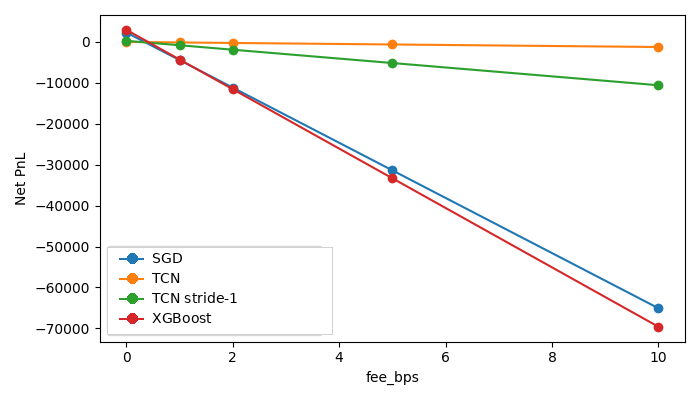
\includegraphics[width=\linewidth]{fig_7_model_fee_stress.png}
\caption{Fee stress curves. Fee stress diagnoses transaction-cost degradation under fixed predictions and thresholds.}
\label{fig:fee_stress}
\end{figure}

Fee stress is the largest reported degradation axis. This pattern is expected in short-horizon LOB replay: the predicted return horizon is small, so increasing fee moves many marginal trades from slightly positive gross edge to negative net edge. For SGD, net PnL changes from $-4{,}437.49$ at 1 bps to $-65{,}082.32$ at 10 bps. XGBoost changes from $-4{,}303.19$ to $-69{,}608.93$, and TCN stride-1 changes from $-814.17$ to $-10{,}587.25$. Latency stress is negative but smaller in the locked grid: at ten latency events, SGD, XGBoost, and TCN stride-1 report $-6{,}096.92$, $-5{,}761.12$, and $-954.59$, respectively.

\begin{figure}[t]
\centering
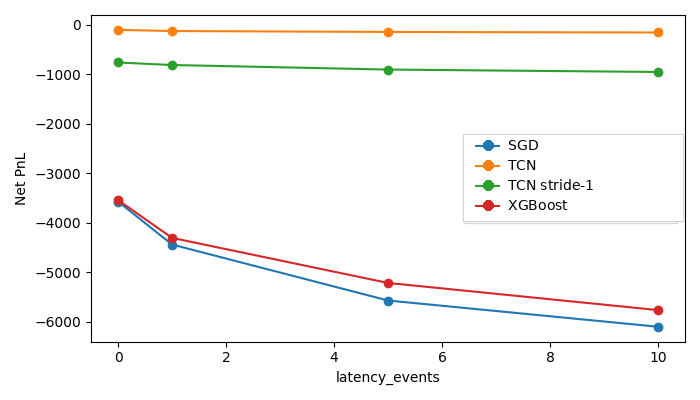
\includegraphics[width=\linewidth]{fig_8_model_latency_stress.png}
\caption{Latency stress curves under the L2 snapshot replay approximation.}
\label{fig:latency_stress}
\end{figure}

\begin{table}[t]
\centering
\caption{Stress-grid endpoints for selected full-test baselines. Values are net PnL; all remain negative.}
\label{tab:stress}
\footnotesize
\begin{tabular}{lrrrr}
\toprule
Model & Fee 10 & Lat. 10 & Spread 2.0 & Depth 0.5 \\
\midrule
SGD & -65,082.32 & -6,096.92 & -4,509.68 & -4,484.19 \\
XGBoost & -69,608.93 & -5,761.12 & -4,418.69 & -4,344.95 \\
TCN stride-1 & -10,587.25 & -954.59 & -819.68 & -818.10 \\
\bottomrule
\end{tabular}
\end{table}

We also summarize each stress axis using a robustness area,
\begin{equation}
\mathrm{RobustnessAUC}_{m,a}=\frac{1}{|\mathcal{L}_a|}\sum_{\ell\in\mathcal{L}_a}\Pi^{\mathrm{net}}_{m,a}(\ell),
\end{equation}
where $\Pi^{\mathrm{net}}_{m,a}(\ell)$ is the net PnL of model $m$ under axis $a$ and stress level $\ell$. Because the main replay is already net negative, more negative values indicate stronger degradation across that stress axis.

The stress summary should be read together with turnover. A model that trades more frequently can accumulate larger total losses even if its per-trade loss is similar. Therefore, robustness summaries are not used to declare a universally superior model; they expose which model-policy combinations are fragile to specific execution assumptions.

\subsection{Worst-Regime Exposure}
Worst-regime diagnostics show that losses concentrate unevenly across regimes. The full RSEP gate has worst-regime return $-64{,}999.54$; removing liquidity risk, adverse-selection risk, or regime penalty gives $-75{,}479.42$, $-70{,}887.92$, and $-69{,}532.74$, respectively. These results suggest that explicit risk components reduce some adverse exposure, but do not eliminate worst-regime losses.

\begin{figure}[t]
\centering
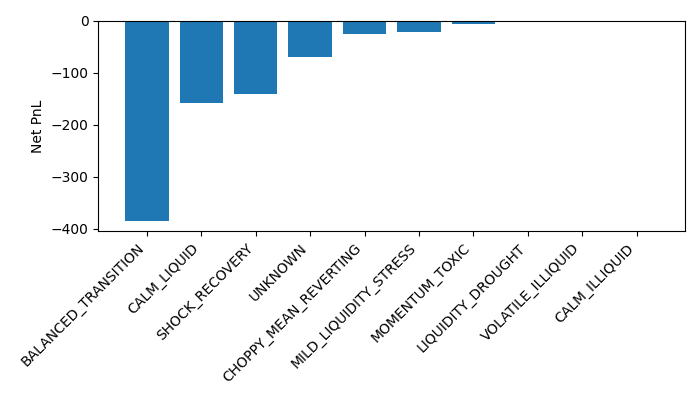
\includegraphics[width=\linewidth]{fig_6_worst_regime.png}
\caption{Worst-regime exposure under selective-execution variants. Worst-regime exposure diagnoses concentration of losses across selective-execution variants.}
\label{fig:worst_regime}
\end{figure}

Failure cases include short actions in regimes such as \texttt{CALM\_LIQUID}, \texttt{MILD\_LIQUIDITY\_STRESS}, \texttt{BALANCED\_TRANSITION}, \texttt{UNKNOWN}, \texttt{CHOPPY\_MEAN\_REVERTING}, and \texttt{SHOCK\_RECOVERY}. Thus, regime labels are useful diagnostics but do not provide oracle-level protection against adverse regimes. The key failure-analysis takeaway is that average forecasting quality can overstate deployable signal, and selective execution can mitigate some exposure without closing the forecast-to-execution gap.

\section{Cross-Asset Evaluation}
\subsection{Protocol and Results}
The asset-held-out protocol trains and tunes on the source asset, then evaluates on the target asset test split without target validation tuning. This prevents using target-specific thresholds to make cross-asset results appear favorable. Table~\ref{tab:cross_asset} reports both directions. BTC$\rightarrow$ETH yields macro-F1 $0.4325$ and MCC $0.1486$; RSEP net PnL is $-74{,}466.38$, compared with $-287{,}991.44$ for cost-aware execution. ETH$\rightarrow$BTC yields macro-F1 $0.4839$ and MCC $0.2424$; RSEP net PnL is $-1{,}144.75$, compared with $-3{,}697.46$ for cost-aware execution.

The two directions are intentionally reported separately. A cross-asset asymmetry audit shows large target/source shifts in price scale, relative spread, visible depth, label mix, regime distribution, and calibration. These diagnostics are consistent with multi-factor distribution shift rather than a single directional cause. Averaging the two directions would hide this asymmetry and could create an overly optimistic transfer narrative. Reporting both directions preserves the failure-analysis framing: the protocol evaluates BTC$\leftrightarrow$ETH transfer under source-validation-only tuning, but it does not imply symmetric transfer quality, universal market generalization, or profitable cross-asset trading.

\begin{table}[t]
\centering
\caption{BTC$\leftrightarrow$ETH asset-held-out evaluation. RSEP reduces losses relative to cost-aware execution in both directions, while absolute net PnL remains negative.}
\label{tab:cross_asset}
\footnotesize
\begin{tabular}{lrrrr}
\toprule
Direction & Macro-F1 & MCC & RSEP net & Cost net \\
\midrule
BTC$\rightarrow$ETH & 0.4325 & 0.1486 & -74,466.38 & -287,991.44 \\
ETH$\rightarrow$BTC & 0.4839 & 0.2424 & -1,144.75 & -3,697.46 \\
\bottomrule
\end{tabular}
\end{table}

\begin{table}[t]
\centering
\caption{Cross-asset bootstrap comparison of RSEP-full minus cost-aware threshold. Positive intervals indicate relative loss mitigation; absolute net PnL remains negative.}
\label{tab:cross_asset_bootstrap}
\footnotesize
\begin{tabular}{lrrrr}
\toprule
Direction & Mean diff. & CI low & CI high & Days \\
\midrule
BTC$\rightarrow$ETH & 3,681.47 & 3,314.02 & 4,048.20 & 58 \\
ETH$\rightarrow$BTC & 39.27 & 34.08 & 44.53 & 65 \\
\bottomrule
\end{tabular}
\end{table}

Day-level bootstrap supports only a relative mitigation claim. For BTC$\rightarrow$ETH, the mean RSEP-minus-cost-aware daily difference is $3{,}681.47$ with CI $[3{,}314.02,4{,}048.20]$. For ETH$\rightarrow$BTC, the mean difference is $39.27$ with CI $[34.08,44.53]$. Both intervals are positive, but absolute net PnL remains negative. The supported generalization is narrow: BTC-USDT and ETH-USDT cross-asset forecasting and execution degradation are evaluated under this protocol; the evidence does not show market-wide transferability, profitability, or readiness for deployment.

\section{Evidence Mapping and Reproducibility}
\subsection{Reproducibility Without Redistributing Commercial Raw Data}
The raw Crypto Lake BTC-USDT and ETH-USDT L2 snapshots are commercial data and are not redistributed, so CryptoRegimeShift-LOB is an artifact-backed benchmark rather than a fully public raw-dataset release. Full numerical reproduction requires licensed snapshots. The public artifact at \url{https://github.com/tvquy85/CryptoRegimeShiftLOB} provides code, configs, schema documentation, synthetic 20-level L2 data, smoke scripts, checksums, split manifests, and paper-ready result artifacts for method-surface audit. Synthetic outputs exercise code paths only and are not used for scientific claims; checksums and manifests link reported tables to specific artifacts.

\begin{table*}[t]
\centering
\caption{Claim-to-evidence map for main paper claims.}
\label{tab:claim_evidence_map}
\scriptsize
\setlength{\tabcolsep}{2pt}
\begin{tabular}{p{0.24\linewidth}p{0.20\linewidth}p{0.24\linewidth}p{0.22\linewidth}}
\toprule
Paper claim & Main evidence & Artifact/check & Limitation \\
\midrule
Forecast metrics do not imply executable value. & Table~\ref{tab:forecasting} + Table~\ref{tab:execution} & Prediction outputs + replay outputs & L2 replay approximation, not live trading \\
RSEP mitigates losses in some settings but does not prove profitability. & Table~\ref{tab:execution} + bootstrap comparison & Daily returns + bootstrap script & Net PnL remains negative \\
Fee stress dominates degradation in the reported grid. & Fig.~\ref{fig:fee_stress} + Table~\ref{tab:stress} & Stress grid CSV & One-axis-at-a-time stress \\
Regime diagnostics reveal concentrated failure modes. & Worst-regime exposure figure/table & By-regime replay results & Diagnostic taxonomy, not latent-state truth \\
BTC$\leftrightarrow$ETH transfer is asymmetric and not universal. & Table~\ref{tab:cross_asset} + Table~\ref{tab:cross_asset_bootstrap} & Cross-asset predictions and replay & Only BTC-USDT and ETH-USDT, Binance 2024 \\
Reproducibility is conditional on licensed raw-data access. & \texttt{DATA\_CARD}, \texttt{SCHEMA}, checksums, sanity-check pipeline & Public supplementary artifact release & Full raw-snapshot reproduction requires licensed access \\
\bottomrule
\end{tabular}
\end{table*}

\section{Threats to Validity}
\subsection{Internal Validity}
The main internal-validity concern is leakage. LOB data are highly autocorrelated, and even small violations of temporal order can inflate both forecasting and execution metrics. The benchmark mitigates this risk by using chronological splits, training-split normalization, validation-only policy tuning, and test-only reporting. Future mid-price values are used only to define labels. They are not used in features, regime assignments, threshold fitting, or execution decisions. The regime taxonomy is likewise time-causal: rolling diagnostics end at the decision time, and quantile thresholds are fitted before test evaluation. These safeguards do not prove that no implementation bug exists, but they define the intended leakage boundary and make it auditable.

A second internal-validity concern is policy overfitting. Because RSEP has several risk weights, it could be over-tuned if thresholds were selected from test results. The paper prevents this by treating validation as the only tuning split and by reporting negative cases. The stride-1 TCN is the most important check here: if the paper had tuned RSEP only to support a favorable narrative, the TCN evidence would likely be omitted. Keeping this result in the main text shows that the benchmark is not optimized to make RSEP appear universally superior.

The artifact package includes a model-selection ledger with feature versions, label versions, threshold grids, validation objectives, selected parameters, and held-out results. We do not claim data-snooping risk is eliminated; instead, we report validation-only selection, test-only reporting, day-level bootstrap, no stress retuning, and retained negative evidence rather than an unsupported overfitting $p$-value.

\subsection{Construct Validity}
Construct validity concerns whether the benchmark measures the intended concept. The target concept is not live trading profit; it is forecast-to-execution degradation under observable L2 frictions. The L2 replay captures spread crossing, visible-depth sweep, explicit fee, latency shift, and stress perturbations. It does not capture hidden liquidity, queue position, order cancellations, market impact beyond the visible-depth approximation, or venue-specific routing. Therefore, net PnL in this paper should be read as a diagnostic quantity produced by a controlled replay approximation. It is useful for comparing degradation under the same assumptions, but it is not a live execution estimate.

The cost-aware label also affects construct validity. If the threshold is too small, the task collapses toward ordinary direction prediction and may overstate actionable signals. If it is too large, many observations become FLAT and the task may understate weak but real predictive structure. The chosen threshold is therefore part of the benchmark definition. The paper reports forecasting metrics, execution results, and stress tests together so that readers can see how this modeling choice propagates into downstream decisions.

\subsection{External Validity}
External validity is intentionally narrow. The benchmark evaluates Binance BTC-USDT and ETH-USDT in 2024. The results should not be generalized to all crypto assets, all venues, equities, futures, or foreign exchange without new experiments. Cross-asset BTC$\leftrightarrow$ETH results strengthen the benchmark relative to a single within-asset split, but they remain two directions inside a related pair of highly liquid crypto markets. Assets with lower liquidity, different fee tiers, different market-making behavior, or different exchange microstructure may produce different degradation profiles.

External validity is also limited by the snapshot frequency and the available depth levels. A higher-frequency message feed, deeper book, or market-by-order dataset could change estimated slippage, latency sensitivity, and passive-fill conclusions. This does not invalidate the benchmark. It means that CryptoRegimeShift-LOB should be viewed as an artifact-backed L2 diagnostic layer. It can be extended when richer data become available, but the present claims remain limited to the L2 snapshot setting.

\subsection{Interpretive Validity}
The final threat is interpretive: readers may be tempted to treat lower losses as success or negative net PnL as failure. Both interpretations are incomplete. Lower losses under RSEP show that selective gates can filter some adverse conditions, but they do not prove profitability. Negative net PnL shows that the forecasting signal is thin after cost and stress, but it does not make the benchmark uninformative. The paper's contribution is precisely to expose this gap. A prediction-only benchmark might stop after reporting macro-F1; CryptoRegimeShift-LOB continues until the signal is mapped through execution, stress, and cross-asset diagnostics.

\section{Discussion}
The practical value of CryptoRegimeShift-LOB is an audit trail from prediction to execution-aware degradation, not a single trading score. Users can ask where a model fails: before costs, after spread crossing, under latency, in a liquidity regime, or under BTC$\leftrightarrow$ETH transfer. Model ranking is evaluation-dependent: accuracy, macro-F1, MCC, and execution diagnostics do not order the baselines identically. The stress grid localizes which execution assumption breaks a signal first, and cross-asset evaluation shows whether the same source-tuned path produces interpretable degradation on a related asset. Future users can add assets, venues, or richer observational layers by rerunning the same evidence path and upgrading claims only when the new data support them.

\section{Limitations and Responsible Use}
CryptoRegimeShift-LOB is bounded by snapshot-level L2 data. This boundary is useful for a public benchmark because visible-depth replay can be specified, tested, stressed, and reused across models. It also defines what the benchmark cannot observe: exact order arrivals, cancellations, queue priority, hidden liquidity, passive-fill dynamics, venue routing, and matching-engine details. Live deployment would require additional venue-specific evidence, including order-routing logs, measured latency, market-impact analysis, operational risk controls, and compliance review.

The forecasting baselines are a controlled diagnostic suite rather than an architecture-leaderboard claim. The execution results remain net negative across main reported policies, which is a core empirical finding of the benchmark: gross directional signal can be overwhelmed by spread crossing, fees, latency, visible-depth constraints, and regime-dependent risk. RSEP is useful as a diagnostic probe because it shows when selective gates reduce exposure or losses and when they fail; the stride-1 TCN is explicit negative evidence because cost-aware execution is better than RSEP and the RSEP-vs-cost-aware bootstrap interval crosses zero.

The regime taxonomy is an evaluation device rather than a true latent-state model. The cross-asset analysis is limited to BTC-USDT$\leftrightarrow$ETH-USDT and should be used as directional transfer evidence, not as a universal cross-market result. The benchmark is intended for research evaluation, robustness analysis, and risk-aware model assessment. It should not be interpreted as investment advice, trading recommendation, or evidence that an automated strategy is ready for deployment. This responsible-use boundary is especially important in crypto markets, where market integrity, liquidity fragmentation, operational risk, and retail exposure remain policy concerns \cite{iosco_crypto2023,fsb2023crypto}.

\section{Conclusion}
This paper introduced CryptoRegimeShift-LOB as a regime-aware L2 crypto benchmark and evaluation protocol for measuring forecast-to-execution degradation. It connects time-causal features, cost-aware labels, interpretable regimes, forecasting baselines, L2 snapshot replay, stress grids, bootstrap diagnostics, and BTC$\leftrightarrow$ETH transfer in one artifact-backed evidence path. The evidence shows that forecast quality and execution usefulness can diverge under costs, stress, regimes, and asset transfer. Negative net PnL is therefore informative evidence: it localizes where apparent forecasting signal is destroyed by observable execution frictions. The significance of CryptoRegimeShift-LOB is the reusable benchmark protocol: credible LOB evaluation should be cost-aware, regime-aware, stress-tested, transfer-aware, and explicit about the limits of snapshot-level L2 data.

\bibliographystyle{IEEEtran}
\bibliography{custom}

\end{document}
